\section{Discussion}
\label{sec:conclusion}

\begin{figure*}[t!]
    \centering
    \subfloat[]{
            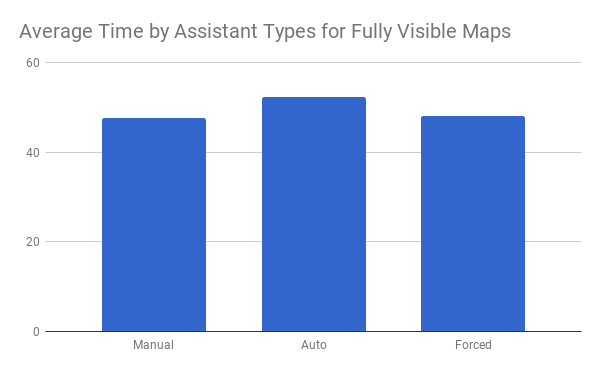
\includegraphics[width=0.33\textwidth]{figs/time_full}
            \label{fig:time_full}
        }
        \subfloat[]{
            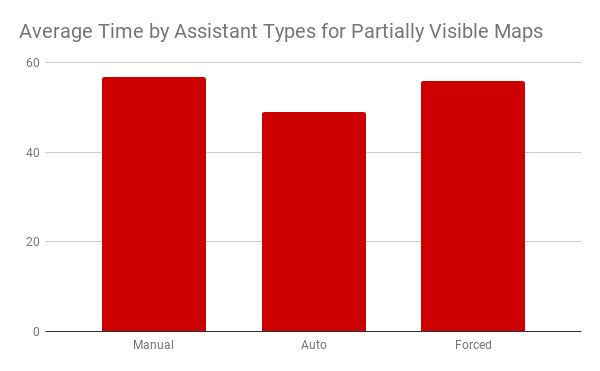
\includegraphics[width=0.33\textwidth]{figs/time_partial} 
            \label{fig:time_partial}
        }
        \subfloat[] {
            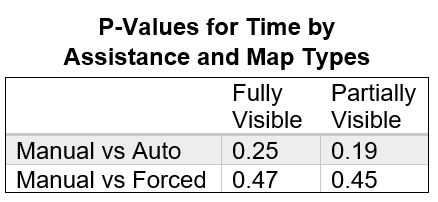
\includegraphics[width=0.33\textwidth]{figs/time_p_values}
            \label{fig:time_p_values}
        }
        \label{fig:charts}
         \caption{\protect\subref{fig:time_full}~The average time taken to complete the task on the fully-visible map for each assistance type. \protect\subref{fig:time_partial}~The average time taken to complete the task on the partially-visible map for each assistance type. \protect\subref{fig:time_p_values}~The p-values for the time taken to complete the task comparing assistance types and map visibility. }
\end{figure*}

\subsubsection{Limitations} 
While our work has shown promising results, there are many limitations to this work. First, users may have potentially learned the map layout even though we changed the goal position. Second, the optimal modes always guided the robot towards the walls users often found this uncomfortable. They did not want to “crawl” along the wall and often changed the mode to move the robot to the middle of the maze. Third, users may have responded differently depending on the randomized order of assistance types. Though all users got the partially visible map first, the assistance type was randomized. Users who got forced assistance early on may have reacted differently to the rest of the maps compared to users who received the manual or automatic assistance type first. Finally, our sample population was not diverse or large enough. Most of our sample size were young females majoring in a STEM field. For more insight, we’d ideally test with a variety of people across different age groups and backgrounds. The current data as it stands is insufficient for us to draw realistic conclusions on how this can be applied outside of this specific user study.

\subsubsection{Future Work}
Even with limitations, there are many possible future directions for this work to explore new concepts and address these limitations. One interesting concept to explore is user trust when the robot provides suboptimal (maximizes mode switches) vs optimal guidance (minimizes mode switches). Our user study only examined user trust when the robot provided optimal assistance. 

Second, we’d also like to extend the algorithm to address the user discomfort with the mode switches that caused the robot to “crawl” along the walls. Ideally, the algorithm would not only optimize for the minimum number of mode switches but would take the user perceptions into account. This extension would allow us to truly understand user trust since the current algorithm’s “lack of optimality” from the user’s perspective may have potentially resulted in a lower comfort rating as reflected in our survey data. 

Third, the ordering of different assistance types can be experimented with. We could potentially address the ordering of assistance types by perhaps fixing the map and assistance type for the first round (after the training map) so that we can establish consistency and better measure user trust. Since we believe this ordering could have impacted user comfort, having a fixed order for part of the study may help us counteract the potential inconsistency and mixed reports on comfort levels. 

Lastly, this work could be extended to run user studies with the Kinova JACO arm. While the 2D interface does mimic the user interface of controlling the JACO arm, to a certain degree, we acknowledge potentially significant impact of leveraging a real robot for user studies. The physical operation of a robot could have impact on emotional comfort or discomfort and attitudes toward robot assistance. 
